\documentclass{ctexart}
\ctexset{
    section = {
        titleformat = \raggedright,
        name = {,、},
        number = \chinese{section}
    }
}
\usepackage[a4paper,top=2.54cm,bottom=2.54cm,left=3.18cm,right=3.18cm]{geometry}
\usepackage{amsmath,amsfonts,amssymb,amsthm}
\usepackage{tikz}
\usepackage{multirow}
\usepackage{array}
\usepackage{fancyhdr}
\usepackage{lastpage}
\usepackage{tabularx}
\usepackage{graphicx}
\usepackage{caption}
\usepackage{pifont}  
\usepackage{xcolor}
%\usepackage{colortbl}  % 添加这一行来支持 \cellcolor
\usepackage{listings}
\usepackage{enumitem}

\definecolor{lightpink}{RGB}{184,83,182}
\definecolor{codebg}{RGB}{245,245,245}
\definecolor{emphcolor}{RGB}{199,21,133}
\definecolor{important}{RGB}{220,20,60}
\definecolor{highlight}{RGB}{0,100,0}
\definecolor{sumregion}{RGB}{255,200,200}
\definecolor{currentcell}{RGB}{255,0,0}

\lstset{
basicstyle=\ttfamily\small,
language=C++,
frame=single,
breaklines=true,
backgroundcolor=\color{codebg},
escapeinside=``,
commentstyle=\color{green!60!black},
keywordstyle=\color{blue},
stringstyle=\color{red},
rulecolor=\color{black},
framesep=5pt,
xleftmargin=10pt,
xrightmargin=10pt
}

\setlist[enumerate,1]{label=\arabic*., leftmargin=2em}
\setlist[enumerate,2]{label=(\arabic*), leftmargin=3em}
\setlist[enumerate,3]{label=\roman*, leftmargin=4em}

\pagestyle{fancy}
\fancyhf{}
\cfoot{解码未来AI教育 \quad 编程题解}
\renewcommand{\headrulewidth}{0pt}

\begin{document}

\section*{二叉树 \ding{78}\ding{78}} 

\subsection*{题目描述}
小杨有一棵包含 $n$ 个节点的二叉树,且根节点的编号为 $1$。这棵二叉树任意一个节点要么是白色,要么是黑色。之后小杨会对这棵二叉树进行 $q$ 次操作,每次小杨会选择一个节点,将以这个节点为根的子树内所有节点的颜色反转,即黑色变成白色,白色变成黑色。

小杨想知道 $q$ 次操作全部完成之后每个节点的颜色。

\subsection*{输入输出格式}

\textbf{输入格式:}
\begin{enumerate}[label={},leftmargin=20pt,itemsep=0pt]
\item 第一行:正整数 $n$,表示节点数量
\item 第二行:$(n-1)$ 个正整数,表示节点 $2$ 到 $n$ 的父亲节点
\item 第三行:长度为 $n$ 的 $01$ 串,表示初始颜色
\item 第四行:正整数 $q$,表示操作次数
\item 接下来 $q$ 行:每行一个正整数 $a_i$,表示操作节点
\end{enumerate}

\textbf{输出格式:}
\begin{enumerate}[label={},leftmargin=20pt,itemsep=0pt]
\item 一行:长度为 $n$ 的 $01$ 串,第 $i$ 位为 $0$ 表示节点 $i$ 为白色,第 $i$ 位为 $1$ 表示节点 $i$ 为黑色
\end{enumerate}


\begin{table}[h]
\centering
\begin{tabularx}{\textwidth}{|X|X|}
\hline
\textbf{输入示例} & \textbf{输出示例}     \\    
\hline
6 & 010000 \\ 
3 1 1 3 4 & \\ 
100101 & \\ 
3 & \\ 
1 & \\ 
3 & \\ 
2 & \\ 
\hline
\end{tabularx}  
\end{table}

\subsection*{样例解释}
\begin{enumerate}
\item \textbf{初始状态}:
\begin{center}
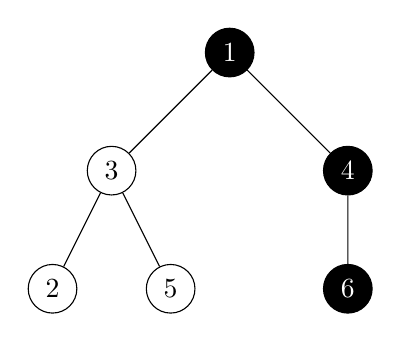
\begin{tikzpicture}[level/.style={sibling distance=30mm/#1}]
\node [circle,draw,fill=black,text=white] (1) {1}
  child { 
    node [circle,draw,fill=white] (3) {3}
    child { node [circle,draw,fill=white] (2) {2} }
    child { node [circle,draw,fill=white] (5) {5} }
  }
  child {
    node [circle,draw,fill=black,text=white] (4) {4}
    child { node [circle,draw,fill=black,text=white] (6) {6} }
  };
\end{tikzpicture}
\end{center}
\begin{itemize}
\item 节点颜色:\textcolor{red}{1(1)}, \textcolor{blue}{2(0)}, \textcolor{blue}{3(0)}, \textcolor{red}{4(1)}, \textcolor{blue}{5(0)}, \textcolor{red}{6(1)}
\item 颜色序列:\texttt{\textcolor{red}{1}\textcolor{blue}{0}\textcolor{blue}{0}\textcolor{red}{1}\textcolor{blue}{0}\textcolor{red}{1}}
\end{itemize}

\item \textbf{第一次操作(节点1)}:
\begin{center}
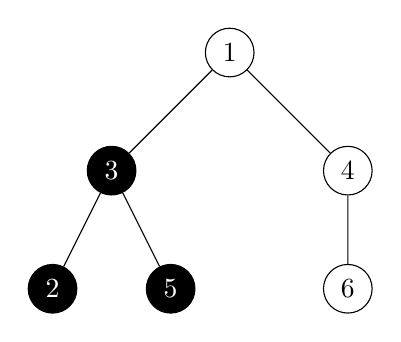
\begin{tikzpicture}[level/.style={sibling distance=30mm/#1}]
\node [circle,draw,fill=white] (1) {1}
  child { 
    node [circle,draw,fill=black,text=white] (3) {3}
    child { node [circle,draw,fill=black,text=white] (2) {2} }
    child { node [circle,draw,fill=black,text=white] (5) {5} }
  }
  child {
    node [circle,draw,fill=white] (4) {4}
    child { node [circle,draw,fill=white] (6) {6} }
  };
\end{tikzpicture}
\end{center}
\begin{itemize}
\item \textcolor{important}{\textbf{反转范围}}:\textcolor{orange}{整个树(所有节点)}
\item 反转后颜色:\textcolor{blue}{1(0)}, \textcolor{red}{2(1)}, \textcolor{red}{3(1)}, \textcolor{blue}{4(0)}, \textcolor{red}{5(1)}, \textcolor{blue}{6(0)}
\item 颜色序列:\texttt{\textcolor{blue}{0}\textcolor{red}{1}\textcolor{red}{1}\textcolor{blue}{0}\textcolor{red}{1}\textcolor{blue}{0}}
\end{itemize}

\item \textbf{第二次操作(节点3)}:
\begin{center}
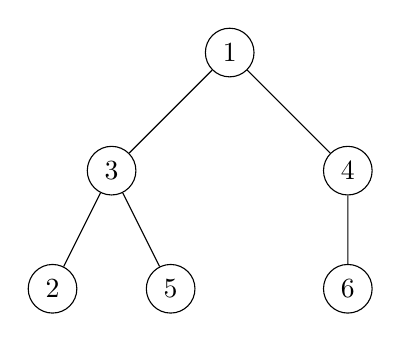
\begin{tikzpicture}[level/.style={sibling distance=30mm/#1}]
\node [circle,draw,fill=white] (1) {1}
  child { 
    node [circle,draw,fill=white] (3) {3}
    child { node [circle,draw,fill=white] (2) {2} }
    child { node [circle,draw,fill=white] (5) {5} }
  }
  child {
    node [circle,draw,fill=white] (4) {4}
    child { node [circle,draw,fill=white] (6) {6} }
  };
\end{tikzpicture}
\end{center}
\begin{itemize}
\item \textcolor{important}{\textbf{反转范围}}:\textcolor{orange}{节点3及其子树(节点3,2,5)}
\item 反转后颜色:\textcolor{blue}{1(0)}, \textcolor{blue}{2(0)}, \textcolor{blue}{3(0)}, \textcolor{blue}{4(0)}, \textcolor{blue}{5(0)}, \textcolor{blue}{6(0)}
\item 颜色序列:\texttt{\textcolor{blue}{0}\textcolor{blue}{0}\textcolor{blue}{0}\textcolor{blue}{0}\textcolor{blue}{0}\textcolor{blue}{0}}
\end{itemize}

\item \textbf{第三次操作(节点2)}:
\begin{center}
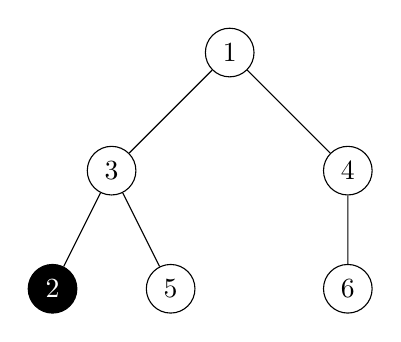
\begin{tikzpicture}[level/.style={sibling distance=30mm/#1}]
\node [circle,draw,fill=white] (1) {1}
  child { 
    node [circle,draw,fill=white] (3) {3}
    child { node [circle,draw,fill=black,text=white] (2) {2} }
    child { node [circle,draw,fill=white] (5) {5} }
  }
  child {
    node [circle,draw,fill=white] (4) {4}
    child { node [circle,draw,fill=white] (6) {6} }
  };
\end{tikzpicture}
\end{center}
\begin{itemize}
\item \textcolor{important}{\textbf{反转范围}}:\textcolor{orange}{节点2(只包含节点2)}
\item 反转后颜色:\textcolor{blue}{1(0)}, \textcolor{red}{2(1)}, \textcolor{blue}{3(0)}, \textcolor{blue}{4(0)}, \textcolor{blue}{5(0)}, \textcolor{blue}{6(0)}
\item 颜色序列:\texttt{\textcolor{blue}{0}\textcolor{red}{1}\textcolor{blue}{0}\textcolor{blue}{0}\textcolor{blue}{0}\textcolor{blue}{0}}
\end{itemize}
\end{enumerate}

\subsection*{背景知识}

在解决树结构相关问题时,图的存储方式至关重要。以下是几种常见的图存储方法:

\begin{enumerate}
\item \textcolor{highlight}{\textbf{邻接矩阵}}
\begin{itemize}
\item 使用二维数组 $graph[i][j]$ 表示节点 $i$ 到节点 $j$ 的边
\item 用 $0$ 表示无边,非 $0$ 表示有边且数值为边的权值
\end{itemize}

\begin{lstlisting}[language=C++]
vector<vector<int>> graph(n + 1, vector<int>(n + 1, 0));
for (int i = 0; i < m; i++) {
    int u, v, w;
    cin >> u >> v >> w;
    graph[u][v] = w;
    graph[v][u] = w; 
}

\end{lstlisting}

\item \textcolor{highlight}{\textbf{邻接表}}
\begin{itemize}
\item 为每个节点维护一个链表,存储该节点的所有相连的节点
\end{itemize}

\begin{lstlisting}[language=C++]
vector<vector<int>> adj(n + 1);
for (int i = 0; i < m; i++) {
    int u, v;
    cin >> u >> v;
    adj[u].push_back(v);
    adj[v].push_back(u);
}
\end{lstlisting}

\item \textcolor{highlight}{\textbf{优缺点对比}}
\begin{table}[h]
\centering
\begin{tabularx}{\textwidth}{|l|X|X|X|X|X|}
\hline
\textbf{存储方式} & \textbf{空间复杂度} & \textbf{查询边(u,v)} & \textbf{遍历邻居} & \textbf{优点} & \textbf{缺点} \\
\hline
邻接矩阵 & $O(n^2)$ & $O(1)$ & $O(n)$ & \begin{tabular}[c]{@{}l@{}}查询速度快\\适合稠密图\end{tabular} & \begin{tabular}[c]{@{}l@{}}空间占用大\\不适合稀疏图\end{tabular} \\
\hline
邻接表 & $O(n+m)$ & $O(\text{deg}(u))$ & $O(\text{deg}(u))$ & \begin{tabular}[c]{@{}l@{}}空间效率高\\适合稀疏图\end{tabular} & \begin{tabular}[c]{@{}l@{}}查询边需遍历\\实现稍复杂\end{tabular} \\
\hline
\end{tabularx}
\end{table}

\end{enumerate}



\subsection*{算法分析}

\begin{enumerate}
\item \textcolor{highlight}{\textbf{直接模拟方法}}\\
对于每次操作,遍历以该节点为根的子树,反转所有节点的颜色 \par
这种方法的时间复杂度为 $O(n \cdot q)$,在 $n,q = 10^5$ 时会超时。

\item \textcolor{highlight}{\textbf{优化方法:标记传递}}\\
利用标记数组记录每个节点被反转的次数,最后统一处理。

\begin{enumerate}
\item \textcolor{highlight}{\textbf{核心思想}}
\begin{itemize}
\item 使用一个标记数组 \texttt{tag} 记录每个节点被反转的次数
\item 对于每次操作,只在操作节点上增加标记
\item 通过一次遍历,将父节点的标记传递给子节点
\item 如果反转次数是奇数,则反转当前节点, 否则不反转
\end{itemize}


\item \textcolor{highlight}{\textbf{算法步骤}}
\begin{itemize}
\item 构建二叉树结构(使用邻接表)
\item 初始化标记数组 \texttt{tag} 为 0
\item 对于每个操作,\texttt{tag[操作节点]++}
\item 使用 BFS 从根节点开始遍历,将父节点的标记累加到子节点
\begin{lstlisting}[language=C++]
queue<pair<int, int>> qu;  `// {当前节点, 父节点}`
qu.push({1, 0});
while (!qu.empty()) {
    int u = qu.front().first;
    int fa = qu.front().second;
    qu.pop();
    
    for (int v : adj[u]) {
        if (v == fa) continue;
        tag[v] += tag[u];
        qu.push({v, u});
    }
}
\end{lstlisting}

\item 计算每个节点的最终颜色
\begin{lstlisting}[language=C++]
for (int i = 1; i <= n; i++) {
    if (tag[i] % 2 == 1) {`// 反转颜色`
    color[i] = (color[i] == '0') ? '1' : '0';
    }
}
\end{lstlisting}

\end{itemize}
\end{enumerate}
\end{enumerate}


\subsection*{拓展思考}
\begin{itemize}
\item 如果颜色的数目修改为k种,且每次操作是将该节点及其子树颜色全部设置为x,那么算法该如何修改?
\item 如果树不是二叉树,而是多叉树,算法是否仍然适用?
\end{itemize}

\end{document}